% Options for packages loaded elsewhere
\PassOptionsToPackage{unicode}{hyperref}
\PassOptionsToPackage{hyphens}{url}
%
\documentclass[
]{book}
\usepackage{amsmath,amssymb}
\usepackage{iftex}
\ifPDFTeX
  \usepackage[T1]{fontenc}
  \usepackage[utf8]{inputenc}
  \usepackage{textcomp} % provide euro and other symbols
\else % if luatex or xetex
  \usepackage{unicode-math} % this also loads fontspec
  \defaultfontfeatures{Scale=MatchLowercase}
  \defaultfontfeatures[\rmfamily]{Ligatures=TeX,Scale=1}
\fi
\usepackage{lmodern}
\ifPDFTeX\else
  % xetex/luatex font selection
\fi
% Use upquote if available, for straight quotes in verbatim environments
\IfFileExists{upquote.sty}{\usepackage{upquote}}{}
\IfFileExists{microtype.sty}{% use microtype if available
  \usepackage[]{microtype}
  \UseMicrotypeSet[protrusion]{basicmath} % disable protrusion for tt fonts
}{}
\makeatletter
\@ifundefined{KOMAClassName}{% if non-KOMA class
  \IfFileExists{parskip.sty}{%
    \usepackage{parskip}
  }{% else
    \setlength{\parindent}{0pt}
    \setlength{\parskip}{6pt plus 2pt minus 1pt}}
}{% if KOMA class
  \KOMAoptions{parskip=half}}
\makeatother
\usepackage{xcolor}
\usepackage{listings}
\newcommand{\passthrough}[1]{#1}
\lstset{defaultdialect=[5.3]Lua}
\lstset{defaultdialect=[x86masm]Assembler}
\usepackage{longtable,booktabs,array}
\usepackage{calc} % for calculating minipage widths
% Correct order of tables after \paragraph or \subparagraph
\usepackage{etoolbox}
\makeatletter
\patchcmd\longtable{\par}{\if@noskipsec\mbox{}\fi\par}{}{}
\makeatother
% Allow footnotes in longtable head/foot
\IfFileExists{footnotehyper.sty}{\usepackage{footnotehyper}}{\usepackage{footnote}}
\makesavenoteenv{longtable}
\usepackage{graphicx}
\makeatletter
\def\maxwidth{\ifdim\Gin@nat@width>\linewidth\linewidth\else\Gin@nat@width\fi}
\def\maxheight{\ifdim\Gin@nat@height>\textheight\textheight\else\Gin@nat@height\fi}
\makeatother
% Scale images if necessary, so that they will not overflow the page
% margins by default, and it is still possible to overwrite the defaults
% using explicit options in \includegraphics[width, height, ...]{}
\setkeys{Gin}{width=\maxwidth,height=\maxheight,keepaspectratio}
% Set default figure placement to htbp
\makeatletter
\def\fps@figure{htbp}
\makeatother
\setlength{\emergencystretch}{3em} % prevent overfull lines
\providecommand{\tightlist}{%
  \setlength{\itemsep}{0pt}\setlength{\parskip}{0pt}}
\setcounter{secnumdepth}{-\maxdimen} % remove section numbering
\ifLuaTeX
  \usepackage{selnolig}  % disable illegal ligatures
\fi
\usepackage{bookmark}
\IfFileExists{xurl.sty}{\usepackage{xurl}}{} % add URL line breaks if available
\urlstyle{same}
\hypersetup{
  hidelinks,
  pdfcreator={LaTeX via pandoc}}

\author{}
\date{}

\begin{document}
\frontmatter

\mainmatter
\begin{lstlisting}[language=Python]
from os.path import basename, exists

def download(url):
    filename = basename(url)
    if not exists(filename):
        from urllib.request import urlretrieve

        local, _ = urlretrieve(url, filename)
        print("Downloaded " + str(local))
    return filename

download('https://raw.githubusercontent.com/AllenDowney/ElementsOfDataScience/v1/utils.py')

import utils

import pandas as pd

# pd.set_option('display.latex.repr', True)

def to_latex(df, *args, **options):
    return df.to_latex(escape=True)

pd.DataFrame._repr_html_ = to_latex

import warnings
warnings.simplefilter(action='ignore', category=FutureWarning)
warnings.simplefilter(action='ignore', category=SyntaxWarning)

import matplotlib.pyplot as plt

# see https://matplotlib.org/stable/users/prev_whats_new/dflt_style_changes.html#figure-size-font-size-and-screen-dpi
plt.rcParams['figure.dpi'] = 300

#plt.rcParams['figure.figsize'] = (6.4, 4.0)
#plt.rcParams['font.size'] = 14
#plt.rcParams['legend.fontsize'] = 14
#plt.rcParams['axes.titlesize'] = 16

# %config InlineBackend.figure_format = 'pdf'
\end{lstlisting}

\chapter{DataFrames and Series}\label{dataframes-and-series}

This chapter introduces Pandas, a Python library that provides functions
for reading and writing data files, exploring and analyzing data, and
generating visualizations. And it provides two new types for working
with data, \passthrough{\lstinline!DataFrame!} and
\passthrough{\lstinline!Series!}.

We will use these tools to answer a data question -- what is the average
birth weight of babies in the United States? This example will
demonstrate important steps in almost any data science project:

\begin{enumerate}
\def\labelenumi{\arabic{enumi}.}
\item
  Identifying data that can answer a question.
\item
  Obtaining the data and loading it in Python.
\item
  Checking the data and dealing with errors.
\item
  Selecting relevant subsets from the data.
\item
  Using histograms to visualize a distribution of values.
\item
  Using summary statistics to describe the data in a way that best
  answers the question.
\item
  Considering possible sources of error and limitations in our
  conclusions.
\end{enumerate}

Let's start by getting the data.

\section{Reading the Data}\label{reading-the-data}

To estimate average birth weight, we'll use data from the National
Survey of Family Growth (NSFG), which is available from the National
Center for Health Statistics. To download the data, you have to agree to
the Data User's Agreement. URLs for the data and the agreement are in
the notebook for this chapter.

You should read the terms carefully, but let me draw your attention to
what I think is the most important one:

\begin{quote}
Make no attempt to learn the identity of any person or establishment
included in these data.
\end{quote}

NSFG respondents answer questions of the most personal nature with the
expectation that their identities will not be revealed. As ethical data
scientists, we should respect their privacy and adhere to the terms of
use.

Respondents to the NSFG provide general information about themselves,
which is stored in the respondent file, and information about each time
they have been pregnant, which is stored in the pregnancy file.

We will work with the pregnancy file, which contains one row for each
pregnancy and one column for each question on the NSFG questionnaire.

The data is stored in a fixed-width format, which means that every row
is the same length and each column spans a fixed range of characters.
For example, the first six characters in each row represent a a unique
identifier for each respondent; the next two characters indicate whether
a pregnancy is the respondent's first, second, etc.

To read this data, we need a \textbf{data dictionary}, which specifies
the names of the columns and the index where each one begins and ends.
The data and the data dictionary are available in separate files.
Instructions for downloading them are in the notebook for this chapter.

\begin{lstlisting}[language=Python]
dict_file = '2015_2017_FemPregSetup.dct'
data_file = '2015_2017_FemPregData.dat'
\end{lstlisting}

Pandas can read data in most common formats, including CSV, Excel, and
fixed-width format, but it cannot read the data dictionary, which is in
Stata format. For that, we'll use a Python library called
\passthrough{\lstinline!statadict!}.

From \passthrough{\lstinline!statadict!}, we'll import
\passthrough{\lstinline!parse\_stata\_dict!}, which reads the data
dictionary.

\begin{lstlisting}[language=Python]
from statadict import parse_stata_dict

stata_dict = parse_stata_dict(dict_file)
stata_dict
\end{lstlisting}

\begin{lstlisting}
<statadict.base.StataDict at 0x7f8afb880f50>
\end{lstlisting}

The result is an object that contains

\begin{itemize}
\item
  \passthrough{\lstinline!names!}, which is a list of column names, and
\item
  \passthrough{\lstinline!colspecs!}, which is a list of tuples, where
  each tuple contains the first and last index of a column.
\end{itemize}

These values are exactly the arguments we need to use
\passthrough{\lstinline!read\_fwf!}, which is the Pandas function that
reads a file in fixed-width format.

\begin{lstlisting}[language=Python]
import pandas as pd

nsfg = pd.read_fwf(data_file, 
                   names=stata_dict.names, 
                   colspecs=stata_dict.colspecs)
type(nsfg)
\end{lstlisting}

\begin{lstlisting}
pandas.core.frame.DataFrame
\end{lstlisting}

The result is a \passthrough{\lstinline!DataFrame!}, which is the
primary type Pandas uses to store data.
\passthrough{\lstinline!DataFrame!} has a method called
\passthrough{\lstinline!head!} that shows the first 5 rows:

\begin{lstlisting}[language=Python]
nsfg.head()
\end{lstlisting}

\begin{tabular}{lrrrrrrrrrrrrrrrrrrrrrrrrrrrrrrrrrrrrrrrrrrrrrrrrrrrrrrrrrrrrrrrrrrrrrrrrrrrrrrrrrrrrrrrrrrrrrrrrrrrrrrrrrrrrrrrrrrrrrrrrrrrrrrrrrrrrrrrrrrrrrrrrrrrrrrrrrrrrrrrrrrrrrrrrrrrrrrrrrrrrrrrrrrrrrrrrrrrrrrrrrrrrrrrrrrrrrrrrrrrrrrrrrrrrrrrrrrrrrrrrrrrrrrrr}
\toprule
 & CASEID & PREGORDR & HOWPREG\_N & HOWPREG\_P & MOSCURRP & NOWPRGDK & PREGEND1 & PREGEND2 & HOWENDDK & NBRNALIV & MULTBRTH & BORNALIV & DATPRGEN\_Y & AGEATEND & HPAGEEND & GESTASUN\_M & GESTASUN\_W & WKSGEST & MOSGEST & DK1GEST & DK2GEST & DK3GEST & BABYSEX1 & BIRTHWGT\_LB1 & BIRTHWGT\_OZ1 & LOBTHWGT1 & BABYSEX2 & BIRTHWGT\_LB2 & BIRTHWGT\_OZ2 & LOBTHWGT2 & BABYSEX3 & BIRTHWGT\_LB3 & BIRTHWGT\_OZ3 & LOBTHWGT3 & BABYDOB\_Y & KIDAGE & HPAGELB & BIRTHPLC & PAYBIRTH1 & PAYBIRTH2 & PAYBIRTH3 & CSECPRIM & CSECMED1 & CSECMED2 & CSECMED3 & CSECMED4 & CSECMED5 & CSECMED6 & CSECPLAN & KNEWPREG & TRIMESTR & LTRIMEST & PRIORSMK & POSTSMKS & NPOSTSMK & GETPRENA & BGNPRENA & PNCTRIM & LPNCTRI & LIVEHERE1 & ALIVENOW1 & WHENDIED\_Y1 & WHENLEFT\_Y1 & LASTAGE1 & WHERENOW1 & LEGAGREE1 & PARENEND1 & ANYNURSE1 & FEDSOLID1 & FRSTEATD\_N1 & FRSTEATD\_P1 & FRSTEATD1 & QUITNURS1 & AGEQTNUR\_N1 & AGEQTNUR\_P1 & AGEQTNUR1 & LIVEHERE2 & ALIVENOW2 & WHENDIED\_Y2 & WHENLEFT\_Y2 & LASTAGE2 & WHERENOW2 & LEGAGREE2 & PARENEND2 & ANYNURSE2 & FEDSOLID2 & FRSTEATD\_N2 & FRSTEATD\_P2 & FRSTEATD2 & QUITNURS2 & AGEQTNUR\_N2 & AGEQTNUR\_P2 & AGEQTNUR2 & LIVEHERE3 & ALIVENOW3 & WHENDIED\_Y3 & WHENLEFT\_Y3 & LASTAGE3 & WHERENOW3 & LEGAGREE3 & PARENEND3 & ANYNURSE3 & FEDSOLID3 & FRSTEATD\_N3 & FRSTEATD\_P3 & FRSTEATD3 & QUITNURS3 & AGEQTNUR\_N3 & AGEQTNUR\_P3 & AGEQTNUR3 & PRGOUTCOME & OUTCOM\_S & NBRNLV\_S & ANYUSINT & EVUSEINT & STOPDUSE & WHYSTOPD & WHATMETH01 & WHATMETH02 & WHATMETH03 & WHATMETH04 & RESNOUSE & WANTBOLD & PROBBABE & CNFRMNO & WANTBLD2 & TIMINGOK & TOOSOON\_N & TOOSOON\_P & WTHPART1 & WTHPART2 & FEELINPG & HPWNOLD & TIMOKHP & COHPBEG & COHPEND & TELLFATH & WHENTELL & TRYSCALE & WANTSCAL & WHYPRG1 & WHYPRG2 & WHYNOUSE1 & WHYNOUSE2 & WHYNOUSE3 & WHYNOUSE4 & WHYNOUSE5 & WHYNOPG1 & WHYNOPG2 & MAINOUSE & PRGLNGTH & OUTCOME & BIRTHORD & DATEND & AGEPREG & DATECON & AGECON & FMAROUT5 & PMARPREG & RMAROUT6 & FMARCON5 & RMARCON6 & LEARNPRG & PNCAREWK & PAYDELIV & LBW1 & LIVCHILD & BFEEDWKS & OLDWANTR & OLDWANTP & WANTRESP & WANTPART & TOOSOON & NEWWANTR & AGER & AGESCRN & FMARITAL & RMARITAL & EDUCAT & HIEDUC & RACE & HISPANIC & HISPRACE & HISPRACE2 & RCURPREG & PREGNUM & PARITY & CURR\_INS & PUBASSIS & POVERTY & LABORFOR & RELIGION & METRO & BRNOUT & YRSTRUS & PRGLNGTH\_I & OUTCOME\_I & BIRTHORD\_I & DATEND\_I & AGEPREG\_I & DATECON\_I & AGECON\_I & FMAROUT5\_I & PMARPREG\_I & RMAROUT6\_I & FMARCON5\_I & RMARCON6\_I & LEARNPRG\_I & PNCAREWK\_I & PAYDELIV\_I & LBW1\_I & LIVCHILD\_I & BFEEDWKS\_I & OLDWANTR\_I & OLDWANTP\_I & WANTRESP\_I & WANTPART\_I & TOOSOON\_I & NEWWANTR\_I & AGER\_I & FMARITAL\_I & RMARITAL\_I & EDUCAT\_I & HIEDUC\_I & RACE\_I & HISPANIC\_I & HISPRACE\_I & HISPRACE2\_I & RCURPREG\_I & PREGNUM\_I & PARITY\_I & CURR\_INS\_I & PUBASSIS\_I & POVERTY\_I & LABORFOR\_I & RELIGION\_I & METRO\_I & WGT2015\_2017 & SECU & SEST & CMINTVW & CMLSTYR & CMJAN3YR & CMJAN4YR & CMJAN5YR & QUARTER & PHASE & INTVWYEAR \\
\midrule
0 & 70627 & 1 & NaN & NaN & NaN & NaN & 6.000000 & NaN & NaN & 1.000000 & NaN & 1.000000 & NaN & NaN & NaN & 0.000000 & 40.000000 & 40.000000 & 9.000000 & NaN & NaN & NaN & 2.000000 & 7.000000 & 8.000000 & NaN & NaN & NaN & NaN & NaN & NaN & NaN & NaN & NaN & 2009.000000 & 6.000000 & 5.000000 & NaN & NaN & NaN & NaN & NaN & NaN & NaN & NaN & NaN & NaN & NaN & NaN & NaN & NaN & NaN & NaN & NaN & NaN & NaN & NaN & NaN & NaN & NaN & NaN & NaN & NaN & NaN & NaN & NaN & NaN & 1.000000 & NaN & 6.000000 & 2.000000 & 1.000000 & NaN & 5.000000 & 1.000000 & 5.000000 & NaN & NaN & NaN & NaN & NaN & NaN & NaN & NaN & NaN & NaN & NaN & NaN & NaN & NaN & NaN & NaN & NaN & NaN & NaN & NaN & NaN & NaN & NaN & NaN & NaN & NaN & NaN & NaN & NaN & NaN & NaN & NaN & NaN & NaN & 1.000000 & 1 & 1.000000 & 1 & 1.000000 & 1.000000 & 1.000000 & NaN & NaN & NaN & NaN & NaN & NaN & NaN & NaN & NaN & 3.000000 & NaN & NaN & 1.000000 & NaN & NaN & 1 & 2.000000 & NaN & NaN & NaN & NaN & NaN & NaN & NaN & NaN & NaN & NaN & NaN & NaN & NaN & NaN & NaN & NaN & 40 & 1 & 1.000000 & 2009.000000 & 29.000000 & 2009 & 28 & 1.000000 & 2.000000 & 1.000000 & 1 & 1 & NaN & NaN & NaN & 2.000000 & 1.000000 & 22.000000 & 1 & 2 & 1 & 2 & NaN & 1 & 35 & 35 & 1 & 1 & 16 & 12 & 2 & 2 & 2 & 2 & 2 & 3 & 2 & 1 & 2 & 500 & 1 & 2 & 1 & 5 & NaN & 0 & 0 & 0 & 0 & 0 & 0 & 0 & 0 & 0 & 0 & 0 & 0 & 0 & 0 & 0 & 0 & 0 & 0 & 0 & 0 & 0 & 0 & 0 & 0 & 0 & 0 & 0 & 0 & 0 & 0 & 0 & 0 & 0 & 0 & 0 & 0 & 0 & 0 & 0 & 0 & 0 & 0 & 19877.457610 & 3 & 322 & 1394 & 1382 & 1357 & 1345 & 1333 & 18 & 1 & 2016 \\
1 & 70627 & 2 & NaN & NaN & NaN & NaN & 1.000000 & NaN & NaN & NaN & NaN & NaN & 2013.000000 & NaN & 5.000000 & 0.000000 & 14.000000 & 14.000000 & 3.000000 & NaN & NaN & NaN & NaN & NaN & NaN & NaN & NaN & NaN & NaN & NaN & NaN & NaN & NaN & NaN & NaN & NaN & NaN & NaN & NaN & NaN & NaN & NaN & NaN & NaN & NaN & NaN & NaN & NaN & NaN & 5.000000 & NaN & NaN & 0.000000 & 5.000000 & NaN & 1.000000 & 10.000000 & NaN & NaN & NaN & NaN & NaN & NaN & NaN & NaN & NaN & NaN & NaN & NaN & NaN & NaN & NaN & NaN & NaN & NaN & NaN & NaN & NaN & NaN & NaN & NaN & NaN & NaN & NaN & NaN & NaN & NaN & NaN & NaN & NaN & NaN & NaN & NaN & NaN & NaN & NaN & NaN & NaN & NaN & NaN & NaN & NaN & NaN & NaN & NaN & NaN & NaN & NaN & NaN & NaN & 2.000000 & 2 & NaN & 5 & NaN & NaN & NaN & NaN & NaN & NaN & NaN & 1.000000 & NaN & NaN & NaN & NaN & 3.000000 & NaN & NaN & 1.000000 & NaN & 10.000000 & 1 & 3.000000 & NaN & NaN & NaN & NaN & 8.000000 & 10.000000 & NaN & NaN & NaN & NaN & NaN & NaN & NaN & NaN & NaN & NaN & 14 & 4 & NaN & 2013.000000 & 32.000000 & 2013 & 32 & 1.000000 & 2.000000 & 1.000000 & 1 & 1 & 5.000000 & 10.000000 & NaN & NaN & NaN & NaN & 1 & 1 & 1 & 1 & NaN & 1 & 35 & 35 & 1 & 1 & 16 & 12 & 2 & 2 & 2 & 2 & 2 & 3 & 2 & 1 & 2 & 500 & 1 & 2 & 1 & 5 & NaN & 0 & 0 & 0 & 0 & 0 & 0 & 0 & 0 & 0 & 0 & 0 & 0 & 0 & 0 & 0 & 0 & 0 & 0 & 0 & 0 & 0 & 0 & 0 & 0 & 0 & 0 & 0 & 0 & 0 & 0 & 0 & 0 & 0 & 0 & 0 & 0 & 0 & 0 & 0 & 0 & 0 & 0 & 19877.457610 & 3 & 322 & 1394 & 1382 & 1357 & 1345 & 1333 & 18 & 1 & 2016 \\
2 & 70627 & 3 & NaN & NaN & NaN & NaN & 6.000000 & NaN & NaN & 1.000000 & NaN & 1.000000 & NaN & NaN & NaN & 0.000000 & 39.000000 & 39.000000 & 9.000000 & NaN & NaN & NaN & 1.000000 & 9.000000 & 2.000000 & NaN & NaN & NaN & NaN & NaN & NaN & NaN & NaN & NaN & 2014.000000 & 1.000000 & 5.000000 & 1.000000 & 1.000000 & 2.000000 & NaN & NaN & NaN & NaN & NaN & NaN & NaN & NaN & NaN & 5.000000 & NaN & NaN & 0.000000 & 5.000000 & NaN & 1.000000 & 10.000000 & NaN & NaN & NaN & NaN & NaN & NaN & NaN & NaN & NaN & NaN & 1.000000 & NaN & 3.000000 & 1.000000 & 3.000000 & 1.000000 & 12.000000 & 1.000000 & 12.000000 & NaN & NaN & NaN & NaN & NaN & NaN & NaN & NaN & NaN & NaN & NaN & NaN & NaN & NaN & NaN & NaN & NaN & NaN & NaN & NaN & NaN & NaN & NaN & NaN & NaN & NaN & NaN & NaN & NaN & NaN & NaN & NaN & NaN & NaN & 1.000000 & 1 & 1.000000 & 5 & NaN & NaN & NaN & NaN & NaN & NaN & NaN & 1.000000 & NaN & NaN & NaN & NaN & 2.000000 & NaN & NaN & 1.000000 & NaN & 10.000000 & 1 & 2.000000 & NaN & NaN & NaN & NaN & 10.000000 & 10.000000 & NaN & NaN & NaN & NaN & NaN & NaN & NaN & NaN & NaN & NaN & 39 & 1 & 2.000000 & 2014.000000 & 33.000000 & 2013 & 33 & 1.000000 & 2.000000 & 1.000000 & 1 & 1 & 5.000000 & 10.000000 & 3.000000 & 2.000000 & 1.000000 & 52.000000 & 2 & 2 & 2 & 2 & NaN & 2 & 35 & 35 & 1 & 1 & 16 & 12 & 2 & 2 & 2 & 2 & 2 & 3 & 2 & 1 & 2 & 500 & 1 & 2 & 1 & 5 & NaN & 0 & 0 & 0 & 0 & 0 & 0 & 0 & 0 & 0 & 0 & 0 & 0 & 0 & 0 & 0 & 0 & 0 & 0 & 0 & 0 & 0 & 0 & 0 & 0 & 0 & 0 & 0 & 0 & 0 & 0 & 0 & 0 & 0 & 0 & 0 & 0 & 0 & 0 & 0 & 0 & 0 & 0 & 19877.457610 & 3 & 322 & 1394 & 1382 & 1357 & 1345 & 1333 & 18 & 1 & 2016 \\
3 & 70628 & 1 & NaN & NaN & NaN & NaN & 6.000000 & NaN & NaN & 1.000000 & NaN & 1.000000 & NaN & NaN & NaN & 9.000000 & 0.000000 & 39.000000 & 9.000000 & NaN & NaN & NaN & 2.000000 & 6.000000 & 9.000000 & NaN & NaN & NaN & NaN & NaN & NaN & NaN & NaN & NaN & 2007.000000 & 6.000000 & 1.000000 & NaN & NaN & NaN & NaN & NaN & NaN & NaN & NaN & NaN & NaN & NaN & NaN & NaN & NaN & NaN & NaN & NaN & NaN & NaN & NaN & NaN & NaN & NaN & NaN & NaN & NaN & NaN & NaN & NaN & NaN & 5.000000 & NaN & NaN & NaN & NaN & NaN & NaN & NaN & NaN & NaN & NaN & NaN & NaN & NaN & NaN & NaN & NaN & NaN & NaN & NaN & NaN & NaN & NaN & NaN & NaN & NaN & NaN & NaN & NaN & NaN & NaN & NaN & NaN & NaN & NaN & NaN & NaN & NaN & NaN & NaN & NaN & NaN & NaN & 1.000000 & 1 & 1.000000 & 1 & 1.000000 & 5.000000 & NaN & 3.000000 & 4.000000 & NaN & NaN & NaN & 5.000000 & NaN & NaN & NaN & NaN & NaN & NaN & NaN & 4.000000 & NaN & 6 & NaN & 5.000000 & 5.000000 & 1.000000 & 1.000000 & NaN & NaN & NaN & NaN & NaN & NaN & NaN & NaN & NaN & NaN & NaN & NaN & 39 & 1 & 1.000000 & 2007.000000 & 18.000000 & 2006 & 17 & 5.000000 & 1.000000 & 6.000000 & 5 & 6 & NaN & NaN & NaN & 2.000000 & 1.000000 & 995.000000 & 5 & 6 & 5 & 6 & NaN & 6 & 28 & 28 & 1 & 1 & 15 & 11 & 1 & 2 & 3 & 3 & 2 & 3 & 3 & 1 & 2 & 189 & 1 & 3 & 1 & 5 & NaN & 0 & 0 & 0 & 0 & 0 & 0 & 0 & 0 & 0 & 0 & 0 & 0 & 0 & 0 & 0 & 0 & 0 & 0 & 0 & 0 & 0 & 0 & 0 & 0 & 0 & 0 & 0 & 0 & 0 & 0 & 0 & 0 & 0 & 0 & 0 & 0 & 0 & 0 & 0 & 0 & 0 & 0 & 4221.017695 & 2 & 366 & 1409 & 1397 & 1369 & 1357 & 1345 & 23 & 1 & 2017 \\
4 & 70628 & 2 & NaN & NaN & NaN & NaN & 6.000000 & NaN & NaN & 1.000000 & NaN & 1.000000 & NaN & NaN & NaN & 9.000000 & 0.000000 & 39.000000 & 9.000000 & NaN & NaN & NaN & 2.000000 & 7.000000 & 0.000000 & NaN & NaN & NaN & NaN & NaN & NaN & NaN & NaN & NaN & 2008.000000 & 6.000000 & 2.000000 & NaN & NaN & NaN & NaN & NaN & NaN & NaN & NaN & NaN & NaN & NaN & NaN & NaN & NaN & NaN & NaN & NaN & NaN & NaN & NaN & NaN & NaN & NaN & NaN & NaN & NaN & NaN & NaN & NaN & NaN & 1.000000 & NaN & 3.000000 & 1.000000 & 3.000000 & NaN & 3.000000 & 1.000000 & 3.000000 & NaN & NaN & NaN & NaN & NaN & NaN & NaN & NaN & NaN & NaN & NaN & NaN & NaN & NaN & NaN & NaN & NaN & NaN & NaN & NaN & NaN & NaN & NaN & NaN & NaN & NaN & NaN & NaN & NaN & NaN & NaN & NaN & NaN & NaN & 1.000000 & 1 & 1.000000 & 5 & 1.000000 & 5.000000 & NaN & 3.000000 & NaN & NaN & NaN & NaN & 1.000000 & NaN & NaN & NaN & 1.000000 & 2.000000 & 2.000000 & NaN & 2.000000 & NaN & 6 & NaN & 1.000000 & 1.000000 & NaN & NaN & NaN & NaN & NaN & NaN & NaN & NaN & NaN & NaN & NaN & NaN & NaN & NaN & 39 & 1 & 2.000000 & 2008.000000 & 20.000000 & 2008 & 19 & 5.000000 & 1.000000 & 5.000000 & 5 & 5 & NaN & NaN & NaN & 2.000000 & 1.000000 & 13.000000 & 3 & 6 & 3 & 6 & 24.000000 & 4 & 28 & 28 & 1 & 1 & 15 & 11 & 1 & 2 & 3 & 3 & 2 & 3 & 3 & 1 & 2 & 189 & 1 & 3 & 1 & 5 & NaN & 0 & 0 & 0 & 0 & 0 & 0 & 0 & 0 & 0 & 0 & 0 & 0 & 0 & 0 & 0 & 0 & 0 & 0 & 0 & 0 & 0 & 0 & 0 & 0 & 0 & 0 & 0 & 0 & 0 & 0 & 0 & 0 & 0 & 0 & 0 & 0 & 0 & 0 & 0 & 0 & 0 & 0 & 4221.017695 & 2 & 366 & 1409 & 1397 & 1369 & 1357 & 1345 & 23 & 1 & 2017 \\
\bottomrule
\end{tabular}

The first two columns are \passthrough{\lstinline!CASEID!} and
\passthrough{\lstinline!PREGORDR!}, which I mentioned earlier. The first
three rows have the same \passthrough{\lstinline!CASEID!}, which means
this respondent reported three pregnancies. The values of
\passthrough{\lstinline!PREGORDR!} indicate that they are the first,
second, and third pregnancies, in that order. We will learn more about
the other columns as we go along.

In addition to methods like \passthrough{\lstinline!head!}, a
\passthrough{\lstinline!Dataframe!} object has several
\textbf{attributes}, which are variables associated with the object. For
example, \passthrough{\lstinline!nsfg!} has an attribute called
\passthrough{\lstinline!shape!}, which is a tuple containing the number
of rows and columns:

\begin{lstlisting}[language=Python]
nsfg.shape
\end{lstlisting}

\begin{lstlisting}
(9553, 248)
\end{lstlisting}

There are 9553 rows in this dataset, one for each pregnancy, and 248
columns, one for each question. \passthrough{\lstinline!nsfg!} also has
an attribute called \passthrough{\lstinline!columns!}, which contains
the column names:

\begin{lstlisting}[language=Python]
nsfg.columns
\end{lstlisting}

\begin{lstlisting}
Index(['CASEID', 'PREGORDR', 'HOWPREG_N', 'HOWPREG_P', 'MOSCURRP', 'NOWPRGDK',
       'PREGEND1', 'PREGEND2', 'HOWENDDK', 'NBRNALIV',
       ...
       'SECU', 'SEST', 'CMINTVW', 'CMLSTYR', 'CMJAN3YR', 'CMJAN4YR',
       'CMJAN5YR', 'QUARTER', 'PHASE', 'INTVWYEAR'],
      dtype='object', length=248)
\end{lstlisting}

The column names are stored in an \passthrough{\lstinline!Index!}, which
is another Pandas type, similar to a list.

Based on the names, you might be able to guess what some of the columns
are, but in general you have to read the documentation. When you work
with datasets like the NSFG, it is important to read the documentation
carefully. If you interpret a column incorrectly, you can generate
nonsense results and never realize it.

So, before we start looking at data, let's get familiar with the NSFG
codebook, which describes every column. Instructions for downloading it
are in the notebook for this chapter.

You can download the codebook for this dataset from
\url{https://github.com/AllenDowney/ElementsOfDataScience/raw/master/data/2015-2017_NSFG_FemPregFile_Codebook-508.pdf}.

If you search that document for ``weigh at birth'' you should find these
columns related to birth weight.

\begin{itemize}
\item
  \passthrough{\lstinline!BIRTHWGT\_LB1!}: Birthweight in Pounds - 1st
  baby from this pregnancy
\item
  \passthrough{\lstinline!BIRTHWGT\_OZ1!}: Birthweight in Ounces - 1st
  baby from this pregnancy
\end{itemize}

There are similar columns for a 2nd or 3rd baby, in the case of twins or
triplets. For now we will focus on the first baby from each pregnancy,
and we will come back to the issue of multiple births.

\section{Series}\label{series}

In many ways a \passthrough{\lstinline!DataFrame!} is like a Python
dictionary, where the column names are the keys and the columns are the
values. You can select a column from a
\passthrough{\lstinline!DataFrame!} using the bracket operator, with a
string as the key.

\begin{lstlisting}[language=Python]
pounds = nsfg['BIRTHWGT_LB1']
type(pounds)
\end{lstlisting}

\begin{lstlisting}
pandas.core.series.Series
\end{lstlisting}

The result is a \passthrough{\lstinline!Series!}, which is a Pandas type
that represents a single column of data. In this case the
\passthrough{\lstinline!Series!} contains the birth weight, in pounds,
for each live birth.

\passthrough{\lstinline!head!} shows the first five values in the
\passthrough{\lstinline!Series!}, the name of the
\passthrough{\lstinline!Series!}, and the data type:

\begin{lstlisting}[language=Python]
pounds.head()
\end{lstlisting}

\begin{lstlisting}
0    7.0
1    NaN
2    9.0
3    6.0
4    7.0
Name: BIRTHWGT_LB1, dtype: float64
\end{lstlisting}

One of the values is \passthrough{\lstinline!NaN!}, which stands for
``Not a Number''. \passthrough{\lstinline!NaN!} is a special value used
to indicate invalid or missing data. In this example, the pregnancy did
not end in live birth, so birth weight is inapplicable.

\textbf{Exercise:} The column \passthrough{\lstinline!BIRTHWGT\_OZ1!}
contains the ounces part of birth weight.

Select the column \passthrough{\lstinline!'BIRTHWGT\_OZ1'!} from
\passthrough{\lstinline!nsfg!} and assign it to a new variable called
\passthrough{\lstinline!ounces!}. Then display the first 5 elements of
\passthrough{\lstinline!ounces!}.

\section{Validation}\label{validation}

At this point we have identified the columns we need to answer the
question and assigned them to variables named
\passthrough{\lstinline!pounds!} and \passthrough{\lstinline!ounces!}.

\begin{lstlisting}[language=Python]
pounds = nsfg['BIRTHWGT_LB1']
ounces = nsfg['BIRTHWGT_OZ1']
\end{lstlisting}

Before we do anything with this data, we have to validate it. One part
of validation is confirming that we are interpreting the data correctly.
We can use the \passthrough{\lstinline!value\_counts!} method to see
what values appear in \passthrough{\lstinline!pounds!} and how many
times each value appears. With \passthrough{\lstinline!dropna=False!},
it includes NaNs. By default, the results are sorted with the highest
count first, but we can use \passthrough{\lstinline!sort\_index!} to
sort them by value instead, with the lightest babies first and heaviest
babies last.

\begin{lstlisting}[language=Python]
pounds.value_counts(dropna=False).sort_index()
\end{lstlisting}

\begin{lstlisting}
BIRTHWGT_LB1
0.0        2
1.0       28
2.0       46
3.0       76
4.0      179
5.0      570
6.0     1644
7.0     2268
8.0     1287
9.0      396
10.0      82
11.0      17
12.0       2
13.0       1
14.0       1
98.0       2
99.0      89
NaN     2863
Name: count, dtype: int64
\end{lstlisting}

The values are in the left column and the counts are in the right
column. The most frequent values are 6-8 pounds, but there are some very
light babies, a few very heavy babies, and two special values, 98, and
99. According to the codebook, these values indicate that the respondent
declined to answer the question (98) or did not know (99).

We can validate the results by comparing them to the codebook, which
lists the values and their frequencies.

\begin{longtable}[]{@{}lll@{}}
\toprule\noalign{}
value & label & Total \\
\midrule\noalign{}
\endhead
\bottomrule\noalign{}
\endlastfoot
. & INAPPLICABLE & 2863 \\
0-5 & UNDER 6 POUNDS & 901 \\
6 & 6 POUNDS & 1644 \\
7 & 7 POUNDS & 2268 \\
8 & 8 POUNDS & 1287 \\
9-95 & 9 POUNDS OR MORE & 499 \\
98 & Refused & 2 \\
99 & Don't know & 89 \\
& Total & 9553 \\
\end{longtable}

The results from \passthrough{\lstinline!value\_counts!} agree with the
codebook, so we can be confident that we are reading and interpreting
the data correctly.

\textbf{Exercise:} In \passthrough{\lstinline!nsfg!}, the
\passthrough{\lstinline!OUTCOME!} column encodes the outcome of each
pregnancy as shown below:

\begin{longtable}[]{@{}ll@{}}
\toprule\noalign{}
Value & Meaning \\
\midrule\noalign{}
\endhead
\bottomrule\noalign{}
\endlastfoot
1 & Live birth \\
2 & Induced abortion \\
3 & Stillbirth \\
4 & Miscarriage \\
5 & Ectopic pregnancy \\
6 & Current pregnancy \\
\end{longtable}

Use \passthrough{\lstinline!value\_counts!} to display the values in
this column and how many times each value appears. Are the results
consistent with the codebook?

\section{Summary Statistics}\label{summary-statistics}

Another way to validate the data is with
\passthrough{\lstinline!describe!}, which computes statistics that
summarize the data, like the mean, standard deviation, minimum, and
maximum. Here are the results for \passthrough{\lstinline!pounds!}.

\begin{lstlisting}[language=Python]
pounds.describe()
\end{lstlisting}

\begin{lstlisting}
count    6690.000000
mean        8.008819
std        10.771360
min         0.000000
25%         6.000000
50%         7.000000
75%         8.000000
max        99.000000
Name: BIRTHWGT_LB1, dtype: float64
\end{lstlisting}

\passthrough{\lstinline!count!} is the number of values, not including
\passthrough{\lstinline!NaN!}. \passthrough{\lstinline!mean!} and
\passthrough{\lstinline!std!} are the mean and standard deviation.
\passthrough{\lstinline!min!} and \passthrough{\lstinline!max!} are the
minimum and maximum values, and in between are the 25th, 50th, and 75th
percentiles. The 50th percentile is the median.

The mean is about 8.05, but that doesn't mean much because it includes
the special values \passthrough{\lstinline!98!} and
\passthrough{\lstinline!99!}. Before we can really compute the mean, we
have to replace those values with \passthrough{\lstinline!NaN!} to
identify them as missing data. The \passthrough{\lstinline!replace!}
method does what we want:

\begin{lstlisting}[language=Python]
import numpy as np

pounds_clean = pounds.replace([98, 99], np.nan)
\end{lstlisting}

\passthrough{\lstinline!replace!} takes a list of the values we want to
replace and the value we want to replace them with.
\passthrough{\lstinline!np.nan!} means we are getting the special value
\passthrough{\lstinline!NaN!} from the NumPy library, which is imported
as \passthrough{\lstinline!np!}. The result is a new
\passthrough{\lstinline!Series!}, which I assign to
\passthrough{\lstinline!pounds\_clean!}. If we run
\passthrough{\lstinline!describe!} again, we see that
\passthrough{\lstinline!count!} is smaller now because it includes only
the valid values.

\begin{lstlisting}[language=Python]
pounds_clean.describe()
\end{lstlisting}

\begin{lstlisting}
count    6599.000000
mean        6.754357
std         1.383268
min         0.000000
25%         6.000000
50%         7.000000
75%         8.000000
max        14.000000
Name: BIRTHWGT_LB1, dtype: float64
\end{lstlisting}

The mean of the new \passthrough{\lstinline!Series!} is about 6.7
pounds. Remember that the mean of the original
\passthrough{\lstinline!Series!} was more than 8 pounds. It makes a big
difference when you remove a few 99-pound babies!

The effect on standard deviation is even more dramatic. If we include
the values \passthrough{\lstinline!98!} and
\passthrough{\lstinline!99!}, the standard deviation is 10.8. If we
remove them -- as we should -- the standard deviation is 1.4.

\textbf{Exercise:} Use \passthrough{\lstinline!describe!} to summarize
\passthrough{\lstinline!ounces!}. Then use
\passthrough{\lstinline!replace!} to replace the special values
\passthrough{\lstinline!98!} and \passthrough{\lstinline!99!} with
\passthrough{\lstinline!NaN!}, and assign the result to
\passthrough{\lstinline!ounces\_clean!}. Run
\passthrough{\lstinline!describe!} again. How much does this cleaning
affect the results?

\section{Series Arithmetic}\label{series-arithmetic}

Now we want to combine \passthrough{\lstinline!pounds!} and
\passthrough{\lstinline!ounces!} into a single
\passthrough{\lstinline!Series!} that contains total birth weight. With
\passthrough{\lstinline!Series!} objects, the arithmetic operators work
elementwise, as they do with NumPy arrays.

So, to convert \passthrough{\lstinline!pounds!} to ounces, we can write
\passthrough{\lstinline!pounds * 16!}. Then, to add in
\passthrough{\lstinline!ounces!} we can write
\passthrough{\lstinline!pounds * 16 + ounces!}.

\textbf{Exercise:} Use \passthrough{\lstinline!pounds\_clean!} and
\passthrough{\lstinline!ounces\_clean!} to compute the total birth
weight expressed in kilograms (there are roughly 2.2 pounds per
kilogram). What is the mean birth weight in kilograms?

\section{Histograms}\label{histograms}

Let's get back to the original question: what is the average birth
weight for babies in the U.S.?\\
As an answer we \emph{could} take the results from the previous section
and compute the mean:

\begin{lstlisting}[language=Python]
pounds_clean = pounds.replace([98, 99], np.nan)
ounces_clean = ounces.replace([98, 99], np.nan)

birth_weight = pounds_clean + ounces_clean / 16
birth_weight.mean()
\end{lstlisting}

\begin{lstlisting}
7.180217889908257
\end{lstlisting}

But it is risky to compute a summary statistic, like the mean, before we
look at the whole distribution of values. A \textbf{distribution} is a
set of possible values and their frequencies. One way to visualize a
distribution is a \textbf{histogram}, which shows values on the x-axis
and their frequencies on the y-axis. \passthrough{\lstinline!Series!}
provides a \passthrough{\lstinline!hist!} method that makes histograms,
and we can use Pyplot to label the axes.

\begin{lstlisting}[language=Python]
import matplotlib.pyplot as plt

birth_weight.hist(bins=30)
plt.xlabel('Birth weight in pounds')
plt.ylabel('Number of live births')
plt.title('Distribution of U.S. birth weight');
\end{lstlisting}

\begin{figure}
\centering
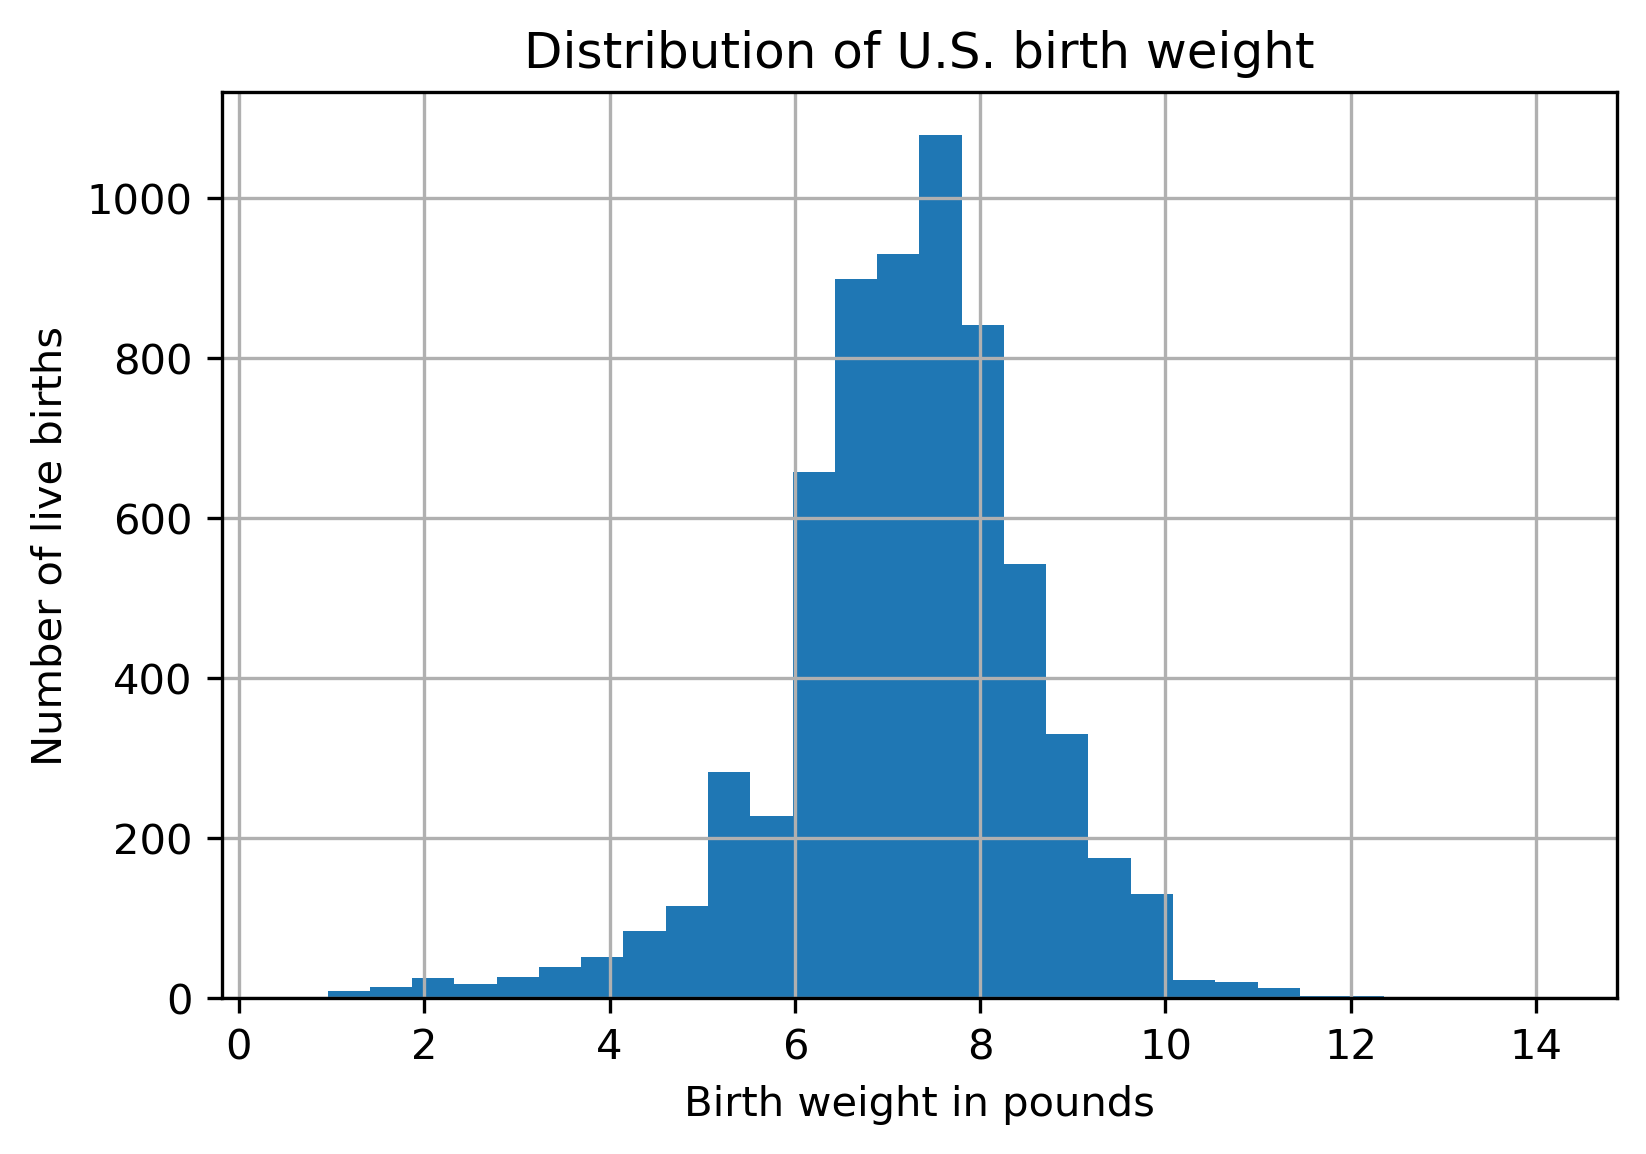
\includegraphics{07_dataframes_files/07_dataframes_60_0.png}
\caption{png}
\end{figure}

The keyword argument, \passthrough{\lstinline!bins!}, tells
\passthrough{\lstinline!hist!} to divide the range of weights into 30
intervals, called \textbf{bins}, and count how many values fall in each
bin. The x-axis is birth weight in pounds; the y-axis is the number of
births in each bin.

The distribution looks like a bell curve, but the tail is longer on the
left than on the right -- that is, there are more light babies than
heavy babies. That makes sense, because the distribution includes some
babies that were born preterm.

\textbf{Exercise:} The NSFG dataset includes a column called
\passthrough{\lstinline!AGECON!} that records a woman's age at
conception for each pregnancy. Select this column from the
\passthrough{\lstinline!DataFrame!} and plot the histogram of the values
with 20 bins. Label the axes and add a title.

\section{Boolean Series}\label{boolean-series}

We have seen that the distribution of birth weights is \textbf{skewed}
to the left -- that is, the left tail extends farther from the center
than the right tail. That's because preterm babies tend to be lighter.
To see which babies are preterm, we can use the
\passthrough{\lstinline!PRGLNGTH!} column, which records pregnancy
length in weeks. A baby is considered preterm if it is born prior to the
37th week of pregnancy.

\begin{lstlisting}[language=Python]
preterm = (nsfg['PRGLNGTH'] < 37)
preterm.dtype
\end{lstlisting}

\begin{lstlisting}
dtype('bool')
\end{lstlisting}

When you compare a \passthrough{\lstinline!Series!} to a value, the
result is a Boolean \passthrough{\lstinline!Series!} -- that is, a
\passthrough{\lstinline!Series!} where each element is a Boolean value,
\passthrough{\lstinline!True!} or \passthrough{\lstinline!False!}. In
this case, it's \passthrough{\lstinline!True!} for each preterm baby and
\passthrough{\lstinline!False!} otherwise. We can use
\passthrough{\lstinline!head!} to see the first 5 elements.

\begin{lstlisting}[language=Python]
preterm.head()
\end{lstlisting}

\begin{lstlisting}
0    False
1     True
2    False
3    False
4    False
Name: PRGLNGTH, dtype: bool
\end{lstlisting}

For a Boolean \passthrough{\lstinline!Series!}, the
\passthrough{\lstinline!sum!} method treats
\passthrough{\lstinline!True!} as 1 and \passthrough{\lstinline!False!}
as 0, so the result is the number of \passthrough{\lstinline!True!}
values, which is the number of preterm babies.

\begin{lstlisting}[language=Python]
preterm.sum()
\end{lstlisting}

\begin{lstlisting}
3675
\end{lstlisting}

If you compute the mean of a Boolean \passthrough{\lstinline!Series!},
the result the \emph{fraction} of \passthrough{\lstinline!True!} values.
In this case, it's about 0.38 -- which means about 38\% of the
pregnancies are less than 37 weeks in duration.

\begin{lstlisting}[language=Python]
preterm.mean()
\end{lstlisting}

\begin{lstlisting}
0.38469590704490736
\end{lstlisting}

However, this result is misleading because it includes all pregnancy
outcomes, not just live births. We can use the
\passthrough{\lstinline!OUTCOME!} column to create another Boolean
\passthrough{\lstinline!Series!} to indicate which pregnancies ended in
live birth.

\begin{lstlisting}[language=Python]
live = (nsfg['OUTCOME'] == 1)
live.mean()
\end{lstlisting}

\begin{lstlisting}
0.7006176070344394
\end{lstlisting}

Now we can use the \passthrough{\lstinline!\&!} operator, which
represents the logical AND operation, to identify pregnancies where the
outcome is a live birth \emph{and} preterm:

\begin{lstlisting}[language=Python]
live_preterm = (live & preterm)
live_preterm.mean()
\end{lstlisting}

\begin{lstlisting}
0.08929132209777034
\end{lstlisting}

About 9\% of all pregnancies resulted in a preterm live birth.

The other common logical operators that work with
\passthrough{\lstinline!Series!} objects are:

\begin{itemize}
\item
  \passthrough{\lstinline!|!}, which represents the logical OR operation
  -- for example, \passthrough{\lstinline!live | preterm!} is true if
  either \passthrough{\lstinline!live!} is true, or
  \passthrough{\lstinline!preterm!} is true, or both.
\item
  \passthrough{\lstinline!\~!}, which represents the logical NOT
  operation -- for example, \passthrough{\lstinline!\~live!} is true if
  \passthrough{\lstinline!live!} not true.
\end{itemize}

The logical operators treat \passthrough{\lstinline!NaN!} the same as
\passthrough{\lstinline!False!}, so you should be careful about using
the NOT operator with a Series that contains
\passthrough{\lstinline!NaN!} values. For example,
\passthrough{\lstinline!\~preterm!} would include not just full term
pregnancies, but also pregnancies with unknown duration.

\textbf{Exercise:} Of all pregnancies, what fraction are live births at
full term (37 weeks or more)? Of all live births, what fraction are full
term?

\section{Filtering Data}\label{filtering-data}

We can use a Boolean \passthrough{\lstinline!Series!} as a filter --
that is, we can select only rows that satisfy a condition or meet some
criterion. For example, we can use \passthrough{\lstinline!preterm!} and
the bracket operator to select values from
\passthrough{\lstinline!birth\_weight!}, so
\passthrough{\lstinline!preterm\_weight!} gets birth weights for preterm
babies.

\begin{lstlisting}[language=Python]
preterm_weight = birth_weight[preterm]
preterm_weight.mean()
\end{lstlisting}

\begin{lstlisting}
5.480958781362007
\end{lstlisting}

To select full-term babies, we can create a Boolean
\passthrough{\lstinline!Series!} like this:

\begin{lstlisting}[language=Python]
fullterm = (nsfg['PRGLNGTH'] >= 37)
\end{lstlisting}

And use it to select birth weights for full term babies:

\begin{lstlisting}[language=Python]
full_term_weight = birth_weight[fullterm]
full_term_weight.mean()
\end{lstlisting}

\begin{lstlisting}
7.429609416096791
\end{lstlisting}

As expected, full term babies are heavier, on average, than preterm
babies. To be more explicit, we could also limit the results to live
births, like this:

\begin{lstlisting}[language=Python]
full_term_weight = birth_weight[live & fullterm]
full_term_weight.mean()
\end{lstlisting}

\begin{lstlisting}
7.429609416096791
\end{lstlisting}

But in this case we get the same result because
\passthrough{\lstinline!birth\_weight!} is only valid for live births.

\textbf{Exercise:} Let's see if there is a difference in weight between
single births and multiple births (twins, triplets, etc.). The column
\passthrough{\lstinline!NBRNALIV!} represents the number of babies born
alive from a single pregnancy.

\begin{lstlisting}[language=Python]
nbrnaliv = nsfg['NBRNALIV']
nbrnaliv.value_counts()
\end{lstlisting}

\begin{lstlisting}
NBRNALIV
1.0    6573
2.0     111
3.0       6
Name: count, dtype: int64
\end{lstlisting}

Use \passthrough{\lstinline!nbrnaliv!} and
\passthrough{\lstinline!live!} to create a Boolean series called
\passthrough{\lstinline!multiple!} that is true for multiple live
births. Of all live births, what fraction are multiple births?

\textbf{Exercise:} Make a Boolean series called
\passthrough{\lstinline!single!} that is true for single live births. Of
all single births, what fraction are preterm? Of all multiple births,
what fraction are preterm?

\textbf{Exercise:} What is the average birth weight for live, single,
full-term births?

\section{Weighted Means}\label{weighted-means}

We are almost done, but there's one more problem we have to solve:
oversampling. The NSFG sample is not exactly representative of the U.S.
population. By design, some groups are more likely to appear in the
sample than others -- that is, they are \textbf{oversampled}.
Oversampling helps to ensure that you have enough people in every group
to get reliable statistics, but it makes data analysis a little more
complicated.

Each pregnancy in the dataset has a \textbf{sampling weight} that
indicates how many pregnancies it represents. In
\passthrough{\lstinline!nsfg!}, the sampling weight is stored in a
column named \passthrough{\lstinline!wgt2015\_2017!}. Here's what it
looks like.

\begin{lstlisting}[language=Python]
sampling_weight = nsfg['WGT2015_2017']
sampling_weight.describe()
\end{lstlisting}

\begin{lstlisting}
count      9553.000000
mean      13337.425944
std       16138.878271
min        1924.916000
25%        4575.221221
50%        7292.490835
75%       15724.902673
max      106774.400000
Name: WGT2015_2017, dtype: float64
\end{lstlisting}

The median value (\passthrough{\lstinline!50!}th percentile) in this
column is about \passthrough{\lstinline!7292!}, which means that a
pregnancy with that weight represents \passthrough{\lstinline!7292!}
total pregnancies in the population. But the range of values is wide, so
some rows represent many more pregnancies than others.

To take these weights into account, we can compute a \textbf{weighted
mean}. Here are the steps:

\begin{enumerate}
\def\labelenumi{\arabic{enumi}.}
\item
  Multiply the birth weights for each pregnancy by the sampling weights
  and add up the products.
\item
  Add up the sampling weights.
\item
  Divide the first sum by the second.
\end{enumerate}

To do this correctly, we have to be careful with missing data. To help
with that, we'll use two \passthrough{\lstinline!Series!} methods,
\passthrough{\lstinline!isna!} and \passthrough{\lstinline!notna!}.
\passthrough{\lstinline!isna!} returns a Boolean
\passthrough{\lstinline!Series!} that is \passthrough{\lstinline!True!}
where the corresponding value is \passthrough{\lstinline!NaN!}.

\begin{lstlisting}[language=Python]
missing = birth_weight.isna()
missing.sum()
\end{lstlisting}

\begin{lstlisting}
3013
\end{lstlisting}

In \passthrough{\lstinline!birth\_weight!} there are
\passthrough{\lstinline!3013!} missing values (mostly for pregnancies
that did not end in live birth). \passthrough{\lstinline!notna!} returns
a Boolean \passthrough{\lstinline!Series!} that is
\passthrough{\lstinline!True!} where the corresponding value is
\emph{not} \passthrough{\lstinline!NaN!}.

\begin{lstlisting}[language=Python]
valid = birth_weight.notna()
valid.sum()
\end{lstlisting}

\begin{lstlisting}
6540
\end{lstlisting}

We can combine \passthrough{\lstinline!valid!} with the other Boolean
\passthrough{\lstinline!Series!} we have computed to identify single,
full term, live births with valid birth weights.

\begin{lstlisting}[language=Python]
single = (nbrnaliv == 1)
selected = valid & live & single & fullterm
selected.sum()
\end{lstlisting}

\begin{lstlisting}
5648
\end{lstlisting}

You can finish off this computation as an exercise.

\textbf{Exercise:} Use \passthrough{\lstinline!selected!},
\passthrough{\lstinline!birth\_weight!}, and
\passthrough{\lstinline!sampling\_weight!} to compute the weighted mean
of birth weight for live, single, full term births. You should find that
the weighted mean is a little higher than the unweighted mean we
computed in the previous section. That's because the groups that are
oversampled in the NSFG tend to have lighter babies, on average.

\section{Making an Extract}\label{making-an-extract}

The NSFG dataset is large, and reading a fixed-width file is relatively
slow. So now that we've read it, let's save a smaller version in a more
efficient format. When we come back to this dataset in Chapter 13, here
are the columns we'll need.

\begin{lstlisting}[language=Python]
variables = ['CASEID', 'OUTCOME', 'BIRTHWGT_LB1', 'BIRTHWGT_OZ1',
             'PRGLNGTH', 'NBRNALIV', 'AGECON', 'AGEPREG', 'BIRTHORD',
             'HPAGELB', 'WGT2015_2017']
\end{lstlisting}

And here's how we can select just those columns from the
\passthrough{\lstinline!DataFrame!}.

\begin{lstlisting}[language=Python]
subset = nsfg[variables]
subset.shape
\end{lstlisting}

\begin{lstlisting}
(9553, 11)
\end{lstlisting}

\passthrough{\lstinline!DataFrame!} provides several methods for writing
data to a file -- the one we'll use is
\passthrough{\lstinline!to\_hdf!}, which creates an HDF file. The
parameters are the name of the new file, the name of the object we're
storing in the file, and the compression level, which determines how
effectively the data are compressed.

\begin{lstlisting}[language=Python]
filename = 'nsfg.hdf'
nsfg.to_hdf(filename, 'nsfg', complevel=6)
\end{lstlisting}

The result is much smaller than the original fixed-width file, and
faster to read. We can read it back like this.

\begin{lstlisting}[language=Python]
nsfg = pd.read_hdf(filename, 'nsfg')
\end{lstlisting}

\section{Summary}\label{summary}

This chapter poses what seems like a simple question: what is the
average birth weight of babies in the United States?

To answer it, we found an appropriate dataset and downloaded the files.
We used Pandas to read the files and create a
\passthrough{\lstinline!DataFrame!}. Then we validated the data and
dealt with special values and missing data. To explore the data, we used
\passthrough{\lstinline!value\_counts!}, \passthrough{\lstinline!hist!},
\passthrough{\lstinline!describe!}, and other methods. And to select
relevant data, we used Boolean \passthrough{\lstinline!Series!} objects.

Along the way, we had to think more about the question. What do we mean
by ``average'', and which babies should we include? Should we include
all live births or exclude preterm babies or multiple births?

And we had to think about the sampling process. By design, the NSFG
respondents are not representative of the U.S. population, but we can
use sampling weights to correct for this effect.

Even a simple question can be a challenging data science project.

A note on vocabulary: In a dataset like the one we used in this chapter,
we could say that each column represents a ``variable'', and what we
called column names might also be called variable names. I avoided that
use of the term because it might be confusing to say that we select a
``variable'' from a \passthrough{\lstinline!DataFrame!} and assign it to
a Python variable. But you might see this use of the term elsewhere, so
I thought I would mention it.

\backmatter
\end{document}
